\section{Testing}
\subsection{Allgemeine Begriffe}
\begin{itemize}
	\item \textbf{\textit{Definition:}} Programm mit der Absicht ausführen, Fehler zu finden. 
	\item Durch das Testen kann die Korrektheit eines Programms aber nicht bewiesen werden! (Ausnahme triviale Programme)
	\item Mit Testen kann nur die Anwesenheit von Bugs bewiesen werden, aber nicht die Abwesenheit. 
	\item Erster Bug: 1947 wurde eine Motte im Relais eines Mark II Aiken Rechners entdeckt.
	\item Nach sorgfältigem Testen steigt die Wahrscheinlichkeit, dass das Programm sich auch in nicht getesteten Fällen wunschgemäss verhält.
\end{itemize}
\begin{multicols}{2}
\subsubsection{Wahrscheinlichkeit von Fehlern}
Je mehr Fehler gefunden werden, desto höher ist die Wahrscheinlichkeit weiterer Fehler.\\
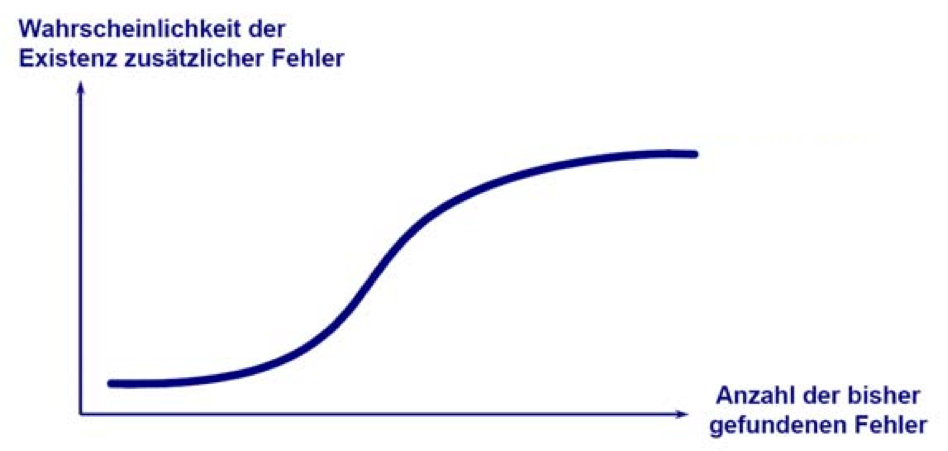
\includegraphics[width=6cm]{images/fehler_wkeit}

	\subsubsection{Verifikation \& Validierung}
	\textbf{Validierung:}\\
	\textit{"{}Are we building the right product?"}\\
	Überprüft das Produkt ob es die Anforderungen des Auftraggebers erfüllt.\\
	\textbf{Verifikation:}\\
	\textit{"{}Are we building the product right?"}\\
	Überprüft ob die erstellte Software funktioniert.\\
	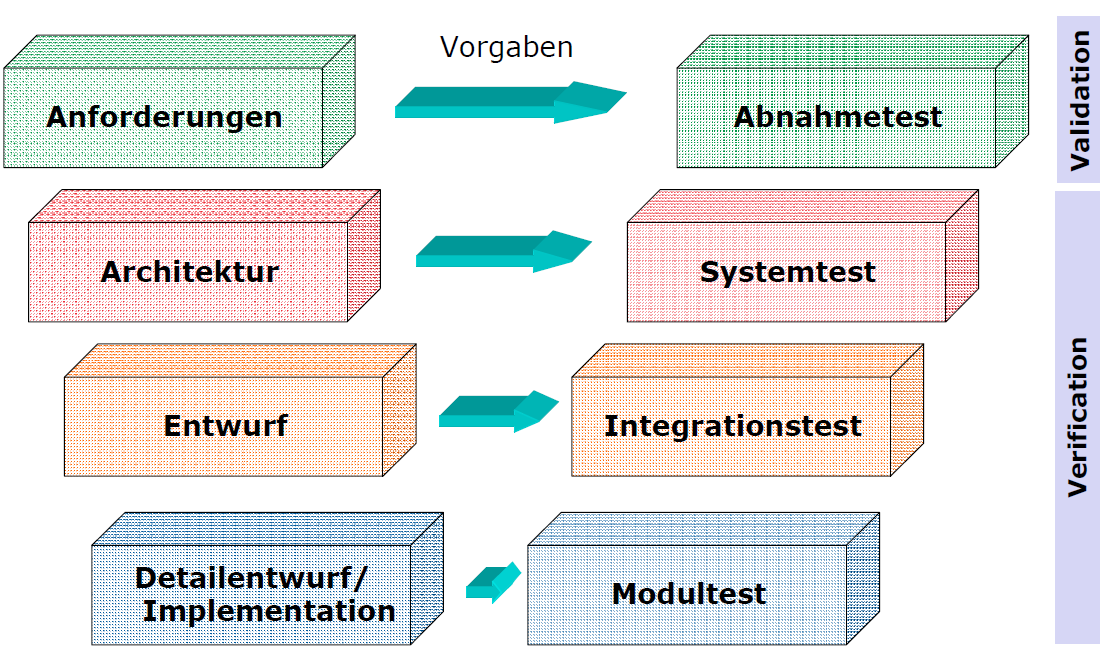
\includegraphics[width=9cm]{images/verificationvalidation}
	
	\subsubsection{Testen \& Debuggen}
	\textbf{Ziel des Testing:} \\
	\begin{minipage}{10cm}
	\vspace{0.2cm}
	\begin{itemize}
		\item Aufzeigen, dass Fehler existieren.
		\item \textit{"{}Jeder gefundene Bug ist ein Gold Nugget"}
	\end{itemize}
	\textbf{Ziel des Debugging:} \\
	Durch Testing gefundene Fehler lokalisieren und beheben.
\end{minipage}

\subsubsection{Anforderungen an Softwaretests}
	\begin{minipage}{12cm}
	\begin{itemize}
			\item Geplant: Testplanung $\rightarrow$ Testplan
			\item Systematisch spezifiziert $\rightarrow$ Testspezifikationen
			\item Testresultate festgehalten $\rightarrow$ Testprotokoll
			\item Reproduzierbarkeit:
			\begin{itemize}
				\item Wissen, was getestet wurde
				\item Unabhängig von testender Person
			\end{itemize}
			\item wenn möglich automatisiert
			\item Testspezifikationen laufend erweitern,\\
			$\Rightarrow$ Regressionstests
		\end{itemize}
	\end{minipage}
		\begin{minipage}{10cm}
			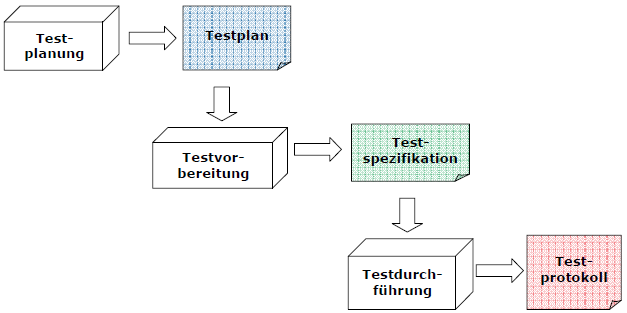
\includegraphics[width=10cm]{images/sofwaretest.png}
		\end{minipage}
\end{multicols}

\begin{multicols}{2}
	\subsubsection{Massnahmen zur Softwareprüfung}
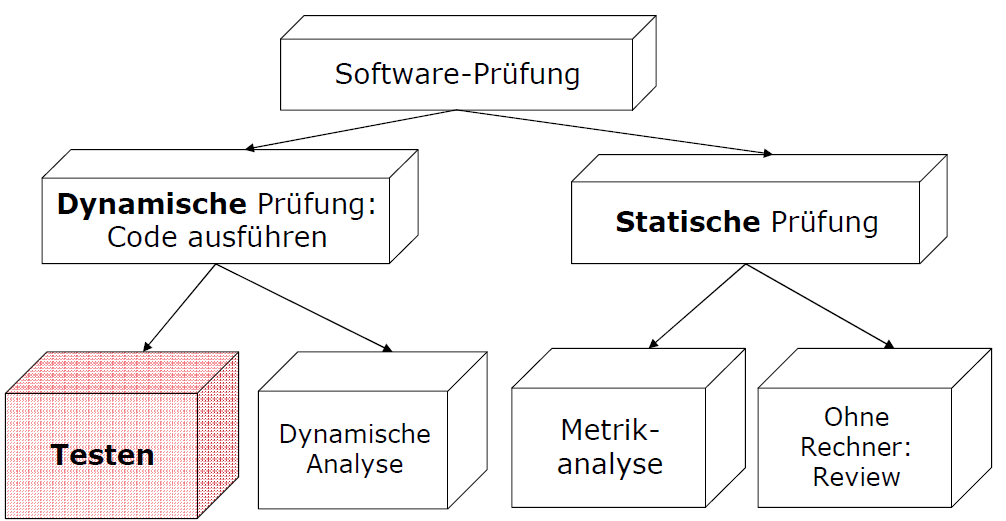
\includegraphics[width = 8cm]{images/massnahmenSoftwarepruefung}
	
	\subsubsection{Arten von Tests}
	\begin{minipage}{10cm}
\begin{tabular}{|p{5cm}|p{4cm}|}
	\hline
	\textbf{Anforderungskategorien} & \textbf{Testkategorien} \\ \hline
	\begin{itemize}
		\item Funktionale Anforderungen
		\item Nichtfunktionale Anforderungen
		\begin{itemize}
			\item Leistung
			\item Usability
			\item ...
		\end{itemize}
		\end{itemize} & 
		\begin{itemize}
		\item Funktionale Tests
		\item Nichtfunktionale Tests
		\begin{itemize}
			\item Leistungstests
			\item Usabilitytests
			\item ...	
		\end{itemize}
	\end{itemize} \\ \hline
\end{tabular}
\end{minipage}
\end{multicols}

\subsection{Testmethoden}
\subsubsection{Testumgebung}
\begin{minipage}{0.5\linewidth}
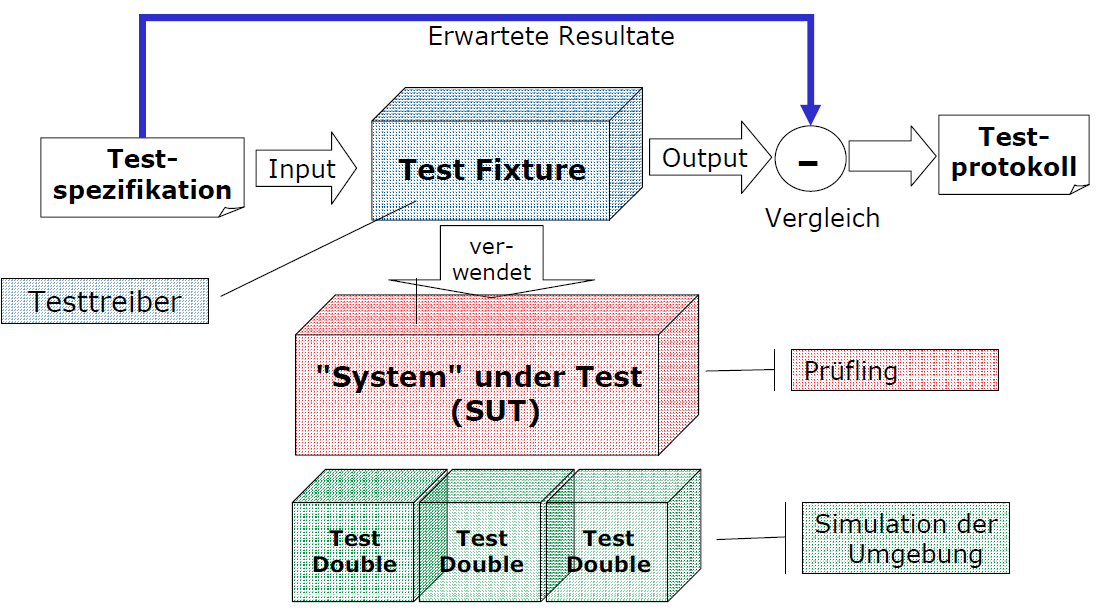
\includegraphics[width=8cm]{images/testumgebung}
\end{minipage}
\begin{minipage}{0.5\linewidth}
	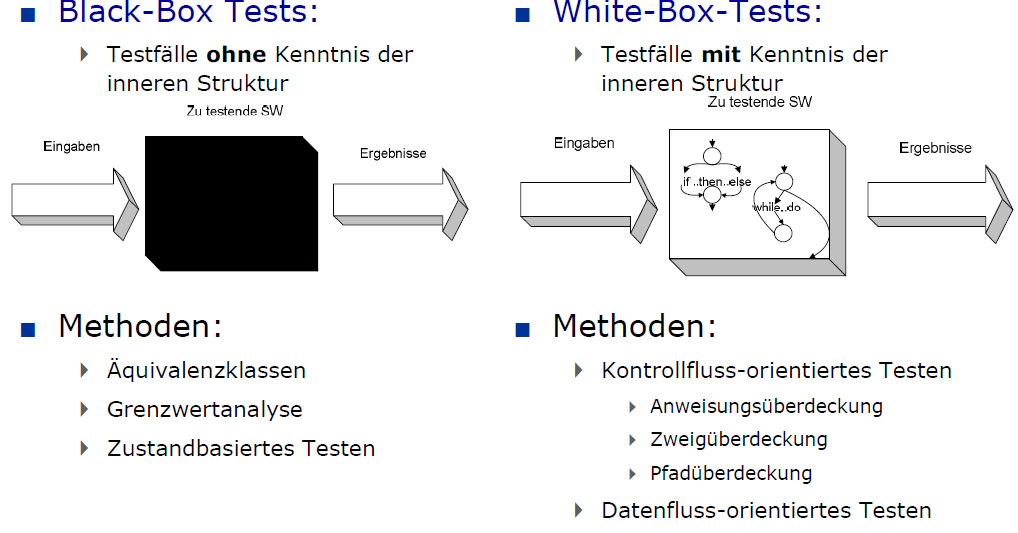
\includegraphics[width=8cm]{images/blackwhitetests}
\end{minipage}
\subsubsection{Blackbox Tests}
Testfälle \textbf{ohne} Kenntnis der inneren Struktur\\\\
\textbf{Äquivalenzklassen:} \\
\begin{minipage}{12cm}
Wertebereich, für welche das Programm voraussichtlich das gleiche Verhalten zeigt. \\
Methodik: 1 Testcase pro Äquivalenzklasse \\
Beispiel: Quadratische Gleichung; Determinante $<0$ ; $=0$ ; $>0$ \\
\vspace{2cm}
\end{minipage}
\begin{minipage}{4cm}
	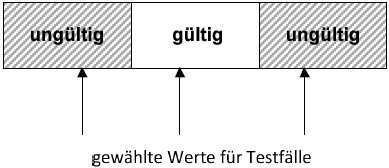
\includegraphics[width=4cm]{images/aequivalenzklasse.png}
\end{minipage}

\textbf{Grenzwertanalyse:} \\
\begin{minipage}{12cm}
Fehler liegen oft an Grenzen zulässiger Eingabewertbereiche. \\
\textit{\textbf{Methodik:}} Testfälle auf Grenzen und knapp daneben \\
\vspace{2cm}
\end{minipage}
\begin{minipage}{4cm}
	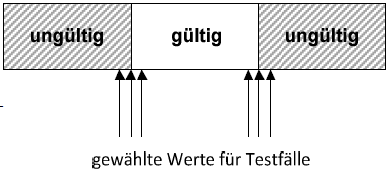
\includegraphics[width=4cm]{images/grenzwertanalyse.png}
\end{minipage}

\textbf{Zustandsbasiertes Testing:} \\
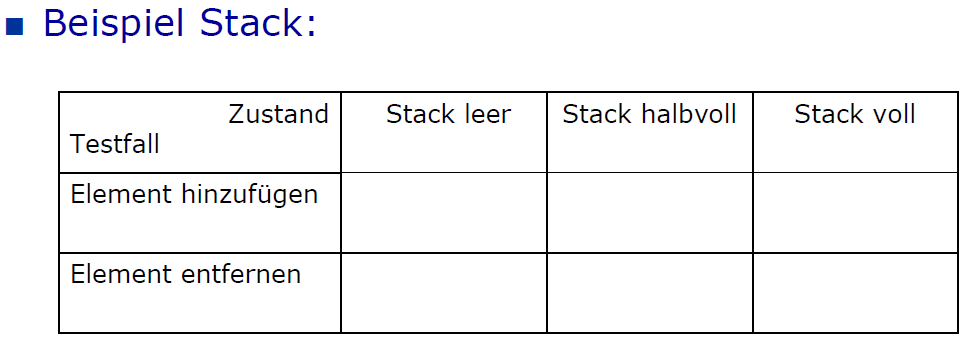
\includegraphics[width = 8cm]{images/stack}
\clearpage
\subsubsection{Whitebox Tests}
\begin{minipage}{8cm}
Tests \textbf{mit} Kenntnis der inneren Struktur\\

\begin{itemize}
\item Whitebox-Test werden mittels Kontrollfluss-Graphen durchgeführt.
\begin{itemize}
	\item Jedes Statement entspricht Knoten.
	\item Zweige, stellen Schleifen und Verzweigungen dar, verbinden Knoten.
\end{itemize}
\item Der Test wird so ausgelegt, dass die Überdeckung (Coverage) möglichst gut ist. (Test der Überdeckung mit Dynamic Analyzer messen)
\end{itemize}
\end{minipage}
\begin{minipage}{7cm}
	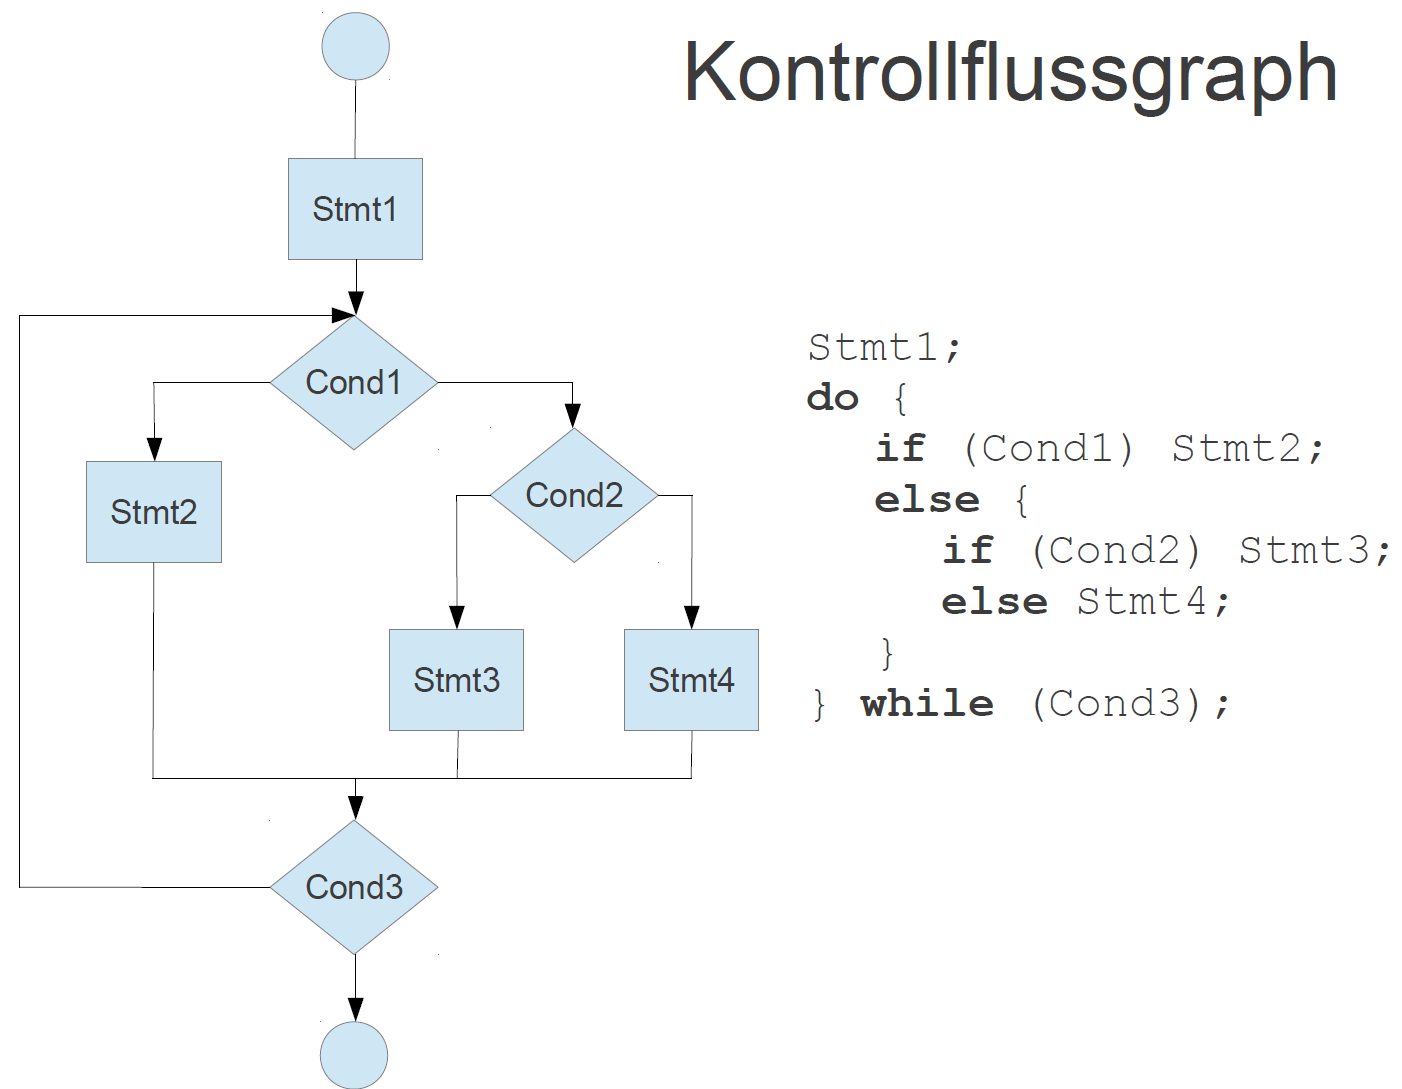
\includegraphics[width=7cm]{images/kontrollflussgraphen.png}
\end{minipage}

\paragraph{Testüberdeckung (test coverage)}
\begin{itemize}
	\item \textbf{\textit{Anweisungsüberdeckung (statement coverage)}}
			\begin{itemize}
				\item Prozentualer Anteil der Anweisungen welche im Test ausgeführt werden
				\item 100\% Anweisungsüberdeckung ist Minimum
			\end{itemize}
	\item \textbf{\textit{Zweigüberdeckung (branch coverage)}}
			\begin{itemize}
				\item Prozentualer Anteil der Zweige welche durchlaufen werden
				\item 100\% Zweigüberdeckung $\Rightarrow$ 100\% Anweisungsüberdeckung
			\end{itemize}
	\item \textbf{\textit{Bedingungsüberdeckung}}
			\begin{itemize}
				\item Verschiedene Kombinationen testen bei zusammengesetzten Bedingungen
				\item mind. 1x true/false durchlaufen
			\end{itemize}
	\item \textbf{\textit{Pfadüberdeckung (path coverage)}}
			\begin{itemize}
				\item Prozentualer Anteil der Pfade welche im Test durchlaufen werden
				\item Ein Pfad ist möglicher Weg durch Kontrollgraphen
			\end{itemize}
	\item \textbf{\textit{Funktionsüberdeckung}}
			\begin{itemize}
				\item \textit{"{}Tut es das, was der Kunde spezifiziert hat?"}
				\item 1 Szenario pro Use Case 
				\item Blackbox Tests
			\end{itemize}
\end{itemize}

\subsection{Testwerkzeuge}
\begin{minipage}{0.5\linewidth}
\begin{tabular}{ll}
	Blackbox: & FIT \\
	Whitebox: & xUnit
\end{tabular}
\\\\
	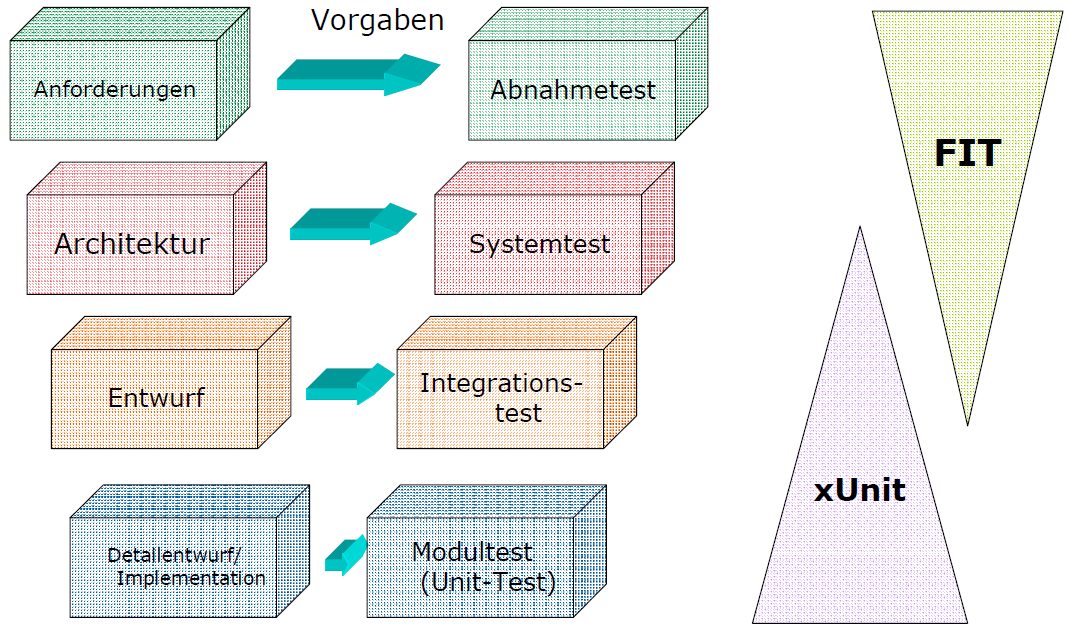
\includegraphics[width=\linewidth]{images/testwerkzeuge}
\end{minipage}
\begin{minipage}{0.5\linewidth}
	\subsection{Wer testet?}
	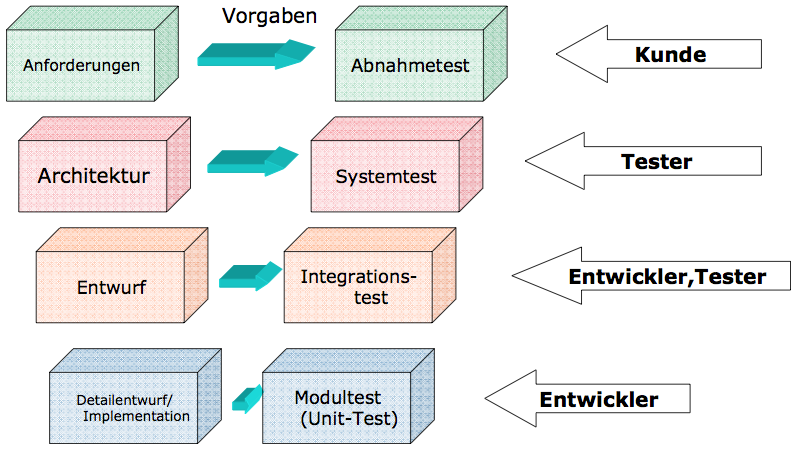
\includegraphics[width=\linewidth]{images/wer_testet}
\end{minipage}
\clearpage

\subsection{Automatisiertes Testing}
\textbf{\textcolor{mygreen}{Vorteile:}}
\begin{itemize}
	\item Wiederholbarkeit \newline $\Rightarrow$ Regressionstests möglich
	\item Eindeutige Spezifikationen (Testcode ist Programmcode)
\end{itemize}	
\textbf{\textcolor{red}{Nachteile:}}
\begin{itemize}
	\item Mehr Code zu schreiben und zu pflegen
	\item Testcode ist Programmcode: Wird überhaupt das Richtige getestet?
\end{itemize}

\subsection{Unit-Test}
\subsubsection{Konzept}
\begin{minipage}{10.5cm}
	\begin{itemize}
		\item Test häufig durch Programmierer selbst
		\item Test einer Komponente (Unit)
		\item Testen der Schnittstelle der Unit
		\item Im Voraus bekannte Ergebnisse $\rightarrow$ Assertions einfügen
		\item automatisch, wiederholbar
		\item heute mittels \textcolor{blue}{\textbf{Unit-Test-Frameworks}} \\
	\textbf{\textit{Frameworks:}} \textcolor{blue}{Programmgerüst} in welches das \textcolor{blue}{Anwendungsprogramm} eingebettet wird. Die Funktionen der Unit werden aus dem Framework heraus aufgerufen, sogenanntes \textbf{Hollywood-Prinzip:}\\\\
		\textit{"{}Don't call us, we'll call you"}
	\end{itemize}
\end{minipage}
\begin{minipage}{9cm}
	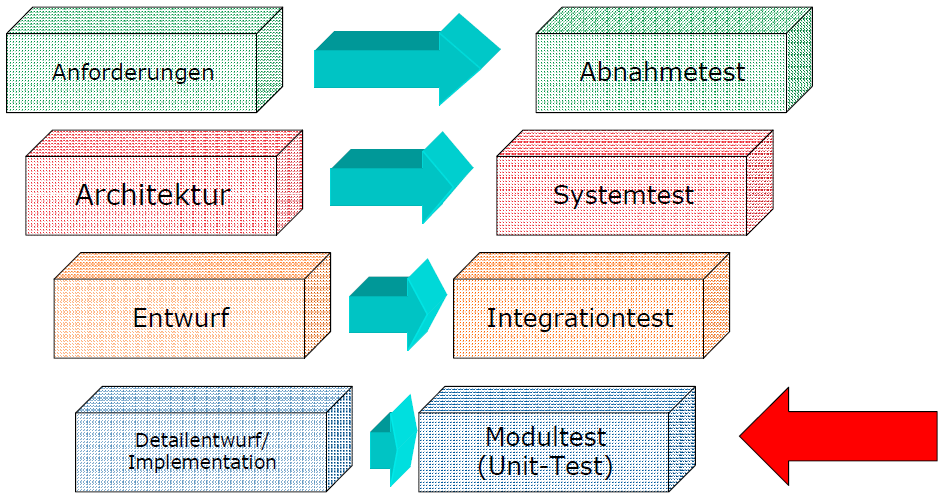
\includegraphics[width=9cm]{images/unittest}
\end{minipage}

\subsubsection{Arbeitsweise}
\begin{itemize}
	\item Spezielle, möglichst einfache Testfunktion mit Zusicherungen
	\begin{itemize}
		\item \texttt{ASSERT(...);} // Vergleicht ein Soll- mit einem Ist-Wert
		\item Stimmen beide überein, ist der Test erfolgreich
		\item Sind sie unterschiedlich $\rightarrow$ Test fehlgeschlagen
	\end{itemize}
	\item Tests laufen automatisiert ab
	\item \textit{Test-Runner} = Programm, das die Test-Funktionen der Reihe nach ausführt
	\begin{itemize}
		\item Test-Run endet mit \"{}OK(...)\"{} oder \"{}FAILED: ...\"{}.
	\end{itemize}
	\item \textbf{Achtung: }
	\begin{itemize}
		\item \texttt{ASSERT(...)} - Anweisungen von Unit-Test nicht mit dem \"{}assert(...)\"{}-Makro aus \"{}assert.h\"{} verwechseln
	\end{itemize}
\end{itemize}

\subsubsection{Unit-Test Frameworks: Vorteile}
\begin{itemize}
	\item Übersichtliche Organisation der Testfälle
	\item Aufteilung der Tests auf mehrere Dateien in der Regel
	\begin{itemize}
		\item Zum Beispiel eine Testklasse pro zu testende Klasse.
	\end{itemize}
	\item Innerhalb der Datei: Organisation der Testfälle in Form von Testfunktionen und Testsuiten.
	\item Automatische Bereitstellung und Abbau einer Testumgebung ist möglich.
	\begin{itemize}
		\item bspw. \texttt{setUp(), tearDown()}
	\end{itemize}
	\item Testprotokolle: Ausgabe der Testergebnisse in verschiedenen Formen möglich. 
\end{itemize}
\begin{multicols}{2}
\subsubsection{CppUnit: Wichtige Begriffe}
\begin{minipage}{8cm}
	\footnotesize{
	\begin{itemize}
		\item \textcolor{blue}{Assert-Anweisung} \newline $\rightarrow$ Zum Vergleich von Ist- und Soll-Wert
		\item \textcolor{blue}{TestKlasse} \newline $\rightarrow$ selbst geschriebene Klasse, die von \"{}CppUnit::TestCase\"{} erbt.
		\item \textcolor{blue}{TestFunktion} \begin{itemize}
			\item enthält Assert-Anweisungen
			\item ist Memberfunktion einer Testklasse
		\end{itemize}
		\item \textcolor{blue}{TestSuite} \newline $\rightarrow$ zur Zusammenfassung von Testfunktionen
		\item \textcolor{blue}{TestFixture} \newline $\rightarrow$ zur Bereitstellung und Abbau einer Testumgebung
		\item \textcolor{blue}{Registry} \newline $\rightarrow$ zur Zusammenfassung von Testklassen
	\end{itemize}}
\end{minipage}
\subsubsection{CppUnit: Testklasse}
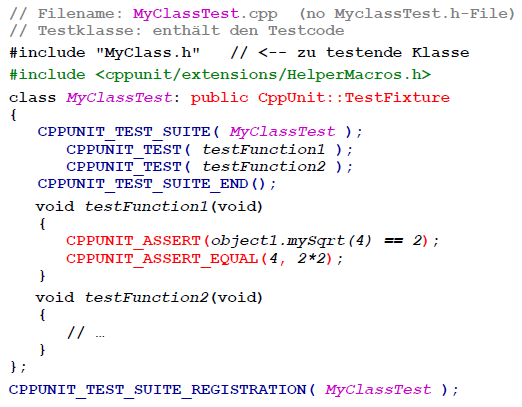
\includegraphics[width = 7cm]{images/testklasse}
\subsubsection{CppUnit: Konventionen}
\begin{itemize}
	\item Für jede zu testende Klasse wird eine entsprechende Testklasse erstellt
	\item Der Name einer Testklasse beginnt mit dem Namen der zu testenden Klasse und endet mit \"{}Test\"{}.
	\item Der Name einer Testfunktion beginnt mit \"{}test\"{}\newline Beispiel: \"{}testAddition()\"{}
\end{itemize} 
\subsubsection{Testprinzipien}
Erst der Test, dann der Code dazu
\subsubsection{Good Unit Tests are \"{}A TRIP\"{}}
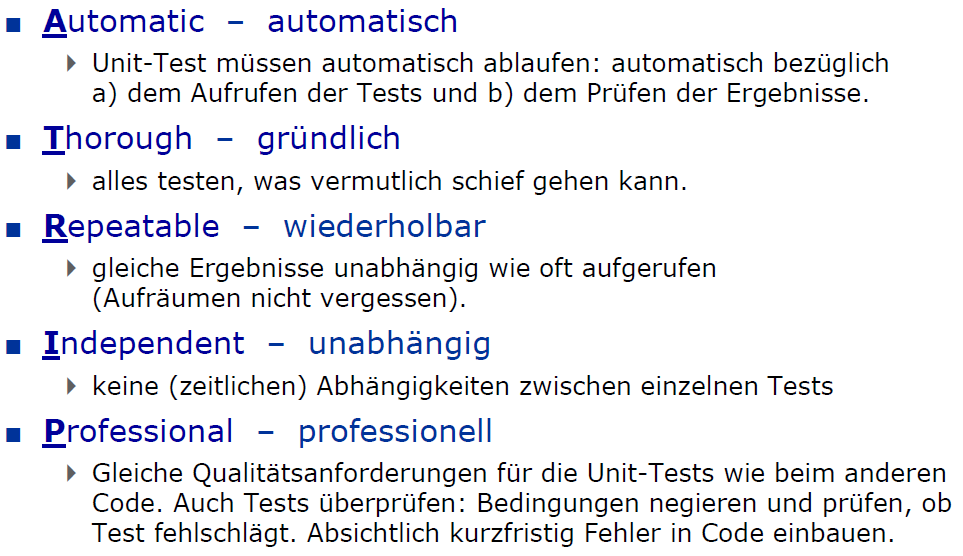
\includegraphics[width=8cm]{images/atrip}
\subsubsection{CORRECT - Boundary Conditions}
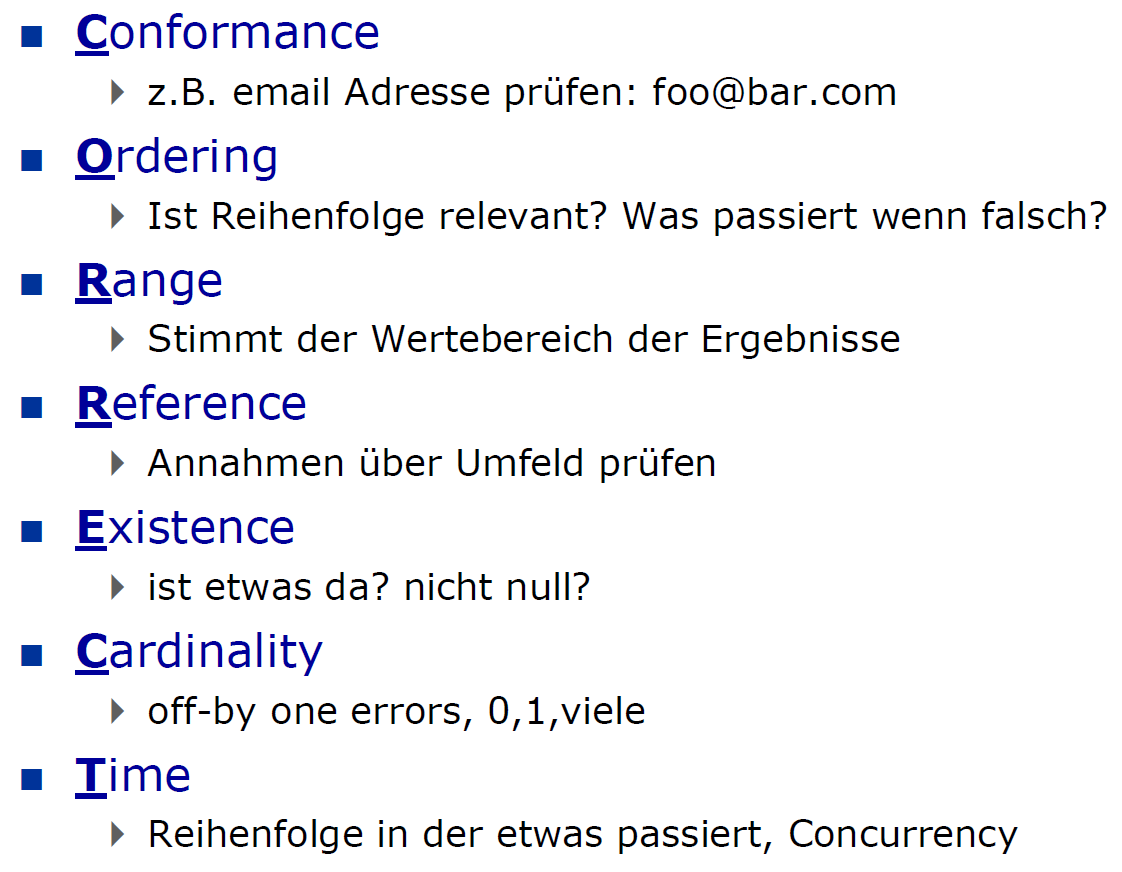
\includegraphics[width=6cm]{images/correct}
\subsubsection{CppUnit: Assert-Makros}
\begin{minipage}{10cm}
\begin{itemize}
\footnotesize{
	\item \textcolor{blue}{\texttt{CPPUNIT\_ASSERT (condition)}}\newline 
	\textcolor{blue}{\texttt{CPPUNIT\_ASSERT\_MESSAGE (msg, condition)}} \newline 
	Test ist okay (d.h. wird bestanden), falls 'condition' true ist.
	\item \textcolor{blue}{\texttt{CPPUNIT\_FAIL (msg)}} \newline
	Test, der immer fehlschlägt.
	\item \textcolor{blue}{\texttt{CPPUNIT\_ASSERT\_EQUAL (expected, actual)}} \newline 
	\textcolor{blue}{\texttt{CPPUNIT\_ASSERT\_EQUAL\_MESSAGE (msg, expected, actual)}} \newline 
	Test ist okay, falls 'expected' und 'actual' gleich sind. Dabei werden einfache Datentypen ('int' etc.) sowie 'std::string' unterstützt.
	\item \textcolor{blue}{\texttt{CPPUNIT\_ASSERT\_DOUBLES\_EQUAL (expected, actual, delta)}} \newline Test ist okay, falls 'expected' und 'actual' innerhalb einer Toleranz von 'delta' gleich sind. Die Argumente sind vom Datentyp 'double'.
	\item \textcolor{blue}{\texttt{CPPUNIT\_ASSERT\_THROW (expression, ExceptionType)}} \newline Test ist okay, falls 'expression' eine Ausnahme vom Typ 'ExceptionType' auslöst.
	\item \textcolor{blue}{\texttt{CPPUNIT\_ASSERT\_NOTHROW (expression)}} \newline 
	Test ist okay, falls 'expression' keine Ausnahme auslöst.
	\item Bei den Varianten mit 'msg' (= message) wird diese zusätzlich ausgegeben, falls der Test fehlschlägt.}
\end{itemize}
\end{minipage}
\subsubsection{Typischer Output}
\footnotesize{
	\textbf{\textit{Suite hat 2 Tests fehlerlos absolviert}}\\
	..\newline \textcolor{red}{\texttt{OK (2)}}\\\\
	\textbf{\textit{Suite hat 10 Tests mit Fehler in Test 2 und 5 absolviert}} \\ 
	...\newline \textcolor{red}{\texttt{MyClassTest.cpp:32:Assertion \newline Test name: MyClassTest::testCtorWithValues\newline equality assertion failed\newline - Expected: 0 \newline - Actual : 15 \newline \newline MyClassTest.cpp:57:Assertion\newline Test name: MyClassTest::testEquals\newline assertion failed\newline - Expression: object.isValid()\newline \newline Failures !!!\newline Run: 10 \qquad Failure total: 2 \qquad Failures: 2 \qquad Errors: 0}}}
\subsubsection{CppUnit Test-Fixture: \texttt{setUp()} und \texttt{tearDown()}}
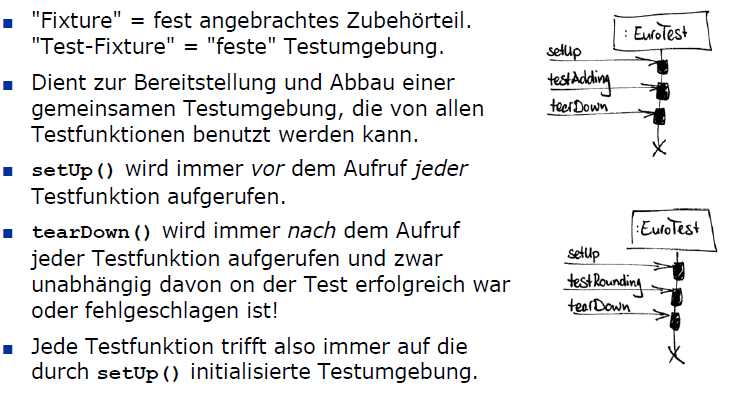
\includegraphics[width = 8 cm]{images/fixture}
\end{multicols}